%!TEX root =conext14.tex
\section{Performance Evaluation}
\label{sec:evaluation}

To evaluate the performance of our proposed system, we implemented our multipath IP in Linux kernel $3.12.1$ under Ubuntu system and install the prototype on two desktops. Both desktops are connected directly to one router without any middle-box. Each desktop has two $100Mbps$ NICs which means that there are totally $4$ paths and the capacity is $200MBps$ between the two nodes. We use Netem\cite{netem} to throttle the connection to evaluate our prototype under multiple scenarios. Wireless connection is also considered in our evaluation.

In all experiments, we try to keep the configuration of each node unchanged after installation. We don't do any special configuration to the system, neither we do any optimization to squeeze out all possible throughput. Except specific experiments that can only be applied to MPIP like UDP experiment and customization MPIP routing, we try to do side-by-side comparison with MPTCP for TCP connections. We will figure out how these two features work independently and together as stated in Section~\ref{sec:together};

For all throughput related experiments, we use iperf3 to generate traffic between the client to the server.


\subsection{Clock Offset}
\label{sec:clock}

During our experiments, we found that the clock of each node has some small difference. In our experiment configuration, the clock of the server is slightly faster than the client. Even this error is very small, we still see the difference in a long experiment.
Certainly, nowadays, most computers have NTP enabled and the system's local time synchronize with time server periodically, but we still think that this difference is worth to be shown here.

On our experiment plat, we turn off NTP on both nodes, do a TCP transmission with iperf3 for one day with consistent traffic. Inside MPIP, we record the one-way delay of each packet from the client to server. Because the traffic load is consistent, queuing delay roughly remains the same. But as shown in Figure~\ref{fig.clock}, because of the clock offset between the two nodes, the trend of queuing delay exposes an linearly increasing curve even the trend is very slow. In Figure~\ref{fig.clock}, we record the queuing delay every one minute. For the whole day($1400$ minutes), we can see that the clock offset is about $350$ milliseconds which means that the server's clock runs one millisecond fast than the client for each four minutes. We will be able to see this trend again in following results.

\begin{figure*}
\centering{
\subfigure[Clock offset
\label{fig.clock}]{\includegraphics[width=0.33\linewidth,height=1.4in]{fig/clock.eps}}
\subfigure[Out-of-order process
\label{fig.outoforder}]{\includegraphics[width=0.33\linewidth,height=1.4in]{fig/out_of_order_w_sack.eps}}
\subfigure[Fake TCP vs UDP Wrapper
\label{fig.implementation}]{\includegraphics[width=0.33\linewidth,height=1.4in]{fig/implementation.eps}}
}
\caption{}
\label{fig.clockandoutoforder}
\end{figure*}


\subsection{TCP Evaluation}
\label{sec:tcp}

As the dominating traffic, TCP plays a critical role in today's Internet. We try to evaluate the performance of MPIP over TCP connections in multiple network configurations. 

\subsubsection{TCP Out-of-order Process}
\label{sec:outoforder}

In Section~\ref{sec:outoforder}, we explained why out-of-order is a problem that must be dealt with in multipath implementations, and we also proposed our solution to this problem. To verify our proposition, we replace one NIC card on the client with a wireless interface. In our experiment plat, the RTT of one path with two wired NICs is about $0.1$ms while paths with one the wireless NIC is about $0.5$ms which will generate enough out-of-order packets. Also, to make sure that there are heavy load of packets to be assigned to the wireless NIC card, instead of using the standard path selection algorithm in Section~\ref{sec:selection}, we fix the weight of all the four paths to be the same. Then we make sure that $50\%$ of outbound packets will be assigned to the wireless NIC.
With this configuration, we do a regular TCP transmission that lasts for $20$ minutes with out-of-order process enabled and disabled respectively. The result is shown in Figure~\ref{fig.outoforder}.

With the same configuration, Figure~\ref{fig.outoforder} shows the improvement brought by the out-of-order process. The average throughput is $XX$Mbps and $XX$Mbps with/out out-of-order process respectively. The improvement maybe trivial if the delay on all the paths is the same because most packets will arrive at the receiver in the order of being sent out. But for multipath connections, it can be very often that each path goes through a totally different route, that is where out-of-order happens most. In all following experiments, we enable out-of-order process by default.

\subsubsection{TCP Throughput Enhancement}
\label{sec:tcptp}

As we mentioned in Section~\ref{sec:tcp}, there are two different implementation of multipath TCP in our system to solve NAT problem which are fake TCP connection and UDP wrapper. We do a specific experiment to evaluate the performance of each approach as shown in Figure~\ref{fig.implementation}. With regular TCP, the average throughput we can achieve is about $92$Mbps. For MPIP, with either fake TCP or UDP wrapper, we both achieve an average throughput of about $165$Mbps. This result shows that both implementations have roughly the same performance. In all following experiments, we use fake TCP by default, but UDP is still kept as an option for users.


Now we start to do side-by-side comparison between MPIP and MPTCP for TCP traffic. Table~\ref{tb.tcp} shows the average throughput comparison results for multiple configurations. 

We first do the transmission without any throttles which means the capacity of the connection is $200$Mbps. We can see that MPIP achieves the highest throughput which is $171$Mbps, MPTCP only gets $129.5$Mbps. When we combine MPIP and MPTCP together as stated in Section~\ref{sec:together}, we get a throughput of $164.6$Mbps.

When we limit the outbound bandwidth of one NIC card on the client to $40$Mbps, we get the result of the second row of Table~\ref{tb.tcp}. In this scenario, the capacity of the connection is $140$Mbps. In this case, MPIP and MPTCP get roughly the same throughput, but when they work together, the highest throughput is achieved.

Besides limiting the outbound bandwidth of one NIC, we also limit the pairwise bandwidth. In this case, we limit the bandwidth from one NIC of the client to the two NICs on the server to $20$Mbps which means the capacity of the connection is still $140$Mbps. In this case, MPIP gets the lowest bandwidth, still, the highest bandwidth is achieved when they work together.

In our experiment plat, with wired connection, the round trip time is trivial(about $0.1$ms). To emulate a connection with more delay, we manually add $5$ms delay to each NIC on the client and get result of the third row in Table~\ref{tb.tcp}. The result is roughly the same as without limit, but we even get higher throughput for MPIP.

By replacing one NIC on the client to a wireless interface, we get the fourth row in Table~\ref{tb.tcp}. In this case, MPTCP achieves higher throughput than MPIP, but still, when they work together, the highest throughput is achieved.


\begin{table}
\caption{\label{tb.tcp}TCP Throughput Comparison}
\centering
\begin{tabular}{|c|c|c|c|}
\hline
  & MPTCP &  MPIP &  MPIP and MPTCP  \\
  & (Mbps) &  (Mbps) &  (Mbps)  \\
\hline
No Limit & $129.5$ & $171.2$ & $164.6$  \\
\hline
NIC BW Limit & $112.6$ & $113.4$ & $125.6$  \\
\hline
Pairwise BW Limit & $114.5$ & $94.7$ & $125.1$  \\
\hline
Delay Limit & $129.7$ & $182.0$ & $165.0$  \\
\hline
Wireless & $97.9$ & $89.2$ & $107.5$  \\
\hline
\end{tabular}
\end{table}

From Figure~\ref{fig.nolimittpcomp} to Figure~\ref{fig.wirelessqdcomp}, we do a analysis among different paths for MPIP transmission to clarify how all packets are assigned to each path. Figure~\ref{fig.nolimittpcomp} to Figure~\ref{fig.wirelessqdcomp} contains four scenarios which refer to the five rows in Table~\ref{tb.tcp} respectively. 

From the throughput comparison results, we can see that even the characters of a path is almost the same, because the coupling of different paths, there can be huge difference in their throughput. In Figure~\ref{fig.nolimittpcomp}, all the four paths are the same, but obviously path $1$ and path $2$ almost take all the traffic. This happens because the four paths are not independent while one NIC is shared by two paths. The queuing delay generated by one path may also affect the queuing delay on the other path. The same explanation can be applied to other throughput comparison results. In Figure~\ref{fig.pairlimittpcomp}, we can see that the two pairwise limited paths don't use all their bandwidth, neither the unlimited two paths, this results in the low throughput for MPIP in this scenario. Figure~\ref{fig.wirelesstpcomp} shows the wireless throughput comparison. The two paths that contains the wireless interface almost get nothing assigned. This is because the high queuing delay of these two paths.

For the queuing delay results, because of the clock offset issue we mentioned in Section~\ref{sec:clock}, we all see a increasing trend. We can calculate the amount of offset during the whole experiment is consistent with the result shown in Figure~\ref{fig.clock}. Generally the queuing delay of wired connection keeps stable once the TCP transmission. For wireless, the fluctuation is very large. In Figure~\ref{fig.delayqdcomp}, we manually add $5$ms delay to each NIC, and also get large but systematic fluctuation, this should be cause by Netem tool that is used to add the delay.


\begin{figure*}[htb]
\centering{
\subfigure[Throughput Comparison without Limit
\label{fig.nolimittpcomp}]{\includegraphics[width=0.24\linewidth,height=1.4in]{fig/no_limit_tp_comp.eps}}
\subfigure[Queuing Delay Comparison without Limit
\label{fig.nolimitqdcomp}]{\includegraphics[width=0.24\linewidth,height=1.4in]{fig/no_limit_qd_comp.eps}}
\subfigure[Throughput Comparison with NIC BW Limit
\label{fig.limittpcomp}]{\includegraphics[width=0.24\linewidth,height=1.4in]{fig/limit_tp_comp.eps}}
\subfigure[Queuing Delay Comparison with NIC BW Limit
\label{fig.limitqdcomp}]{\includegraphics[width=0.24\linewidth,height=1.4in]{fig/limit_qd_comp.eps}}
\subfigure[Throughput Comparison with Pairwise BW Limit
\label{fig.pairlimittpcomp}]{\includegraphics[width=0.24\linewidth,height=1.4in]{fig/pair_limit_tp_comp.eps}}
\subfigure[Queuing Delay Comparison with Pairwise BW Limit
\label{fig.pairlimitqdcomp}]{\includegraphics[width=0.24\linewidth,height=1.4in]{fig/pair_limit_qd_comp.eps}}
\subfigure[Throughput Comparison with additional delay
\label{fig.delaytpcomp}]{\includegraphics[width=0.24\linewidth,height=1.4in]{fig/delay_tp_comp.eps}}
\subfigure[Queuing Delay Comparison with additional delay
\label{fig.delayqdcomp}]{\includegraphics[width=0.24\linewidth,height=1.4in]{fig/delay_qd_comp.eps}}
\subfigure[Throughput Comparison for wireless
\label{fig.wirelesstpcomp}]{\includegraphics[width=0.24\linewidth,height=1.4in]{fig/wireless_tp_comp.eps}}
\subfigure[Queuing Delay Comparison for wireless
\label{fig.wirelessqdcomp}]{\includegraphics[width=0.24\linewidth,height=1.4in]{fig/wireless_qd_comp.eps}}
\subfigure[Throughput Comparison for two paths
\label{fig.twopathstpcomp}]{\includegraphics[width=0.24\linewidth,height=1.4in]{fig/twopaths_tp_comp.eps}}
\subfigure[Queuing Delay Comparison for two paths
\label{fig.twopathsqdcomp}]{\includegraphics[width=0.24\linewidth,height=1.4in]{fig/twopaths_qd_comp.eps}}
}
\caption{MPIP Path Comparison}
\label{fig.mpip_path}
\end{figure*}

Besides using all four paths, we also limit the number of path to two. Also we limit the bandwidth of one path to $40$Mbps which makes the capacity $140$Mbps on the connection. Figure~\ref{fig.twopathstpcomp} and Figure~\ref{fig.twopathsqdcomp} shows the throughput and queuing delay result for this configuration. The result we get here is roughly the same as in Figure~\ref{fig.pairlimittpcomp} and Figure~\ref{fig.pairlimitqdcomp}.


Besides the controlled lab experiments, we also evaluate MPIP on the Internet to verify the prototype's NAT immunization and system robustness. We set up our server at Emulab which is located in Utah while the client is in New York. Because there is only one NIC that connects to Internet on the Emulab node, there are only $2$ paths in this case. According to our test, the capacity between our client and the server in Emulab is about $5Mbps$. Also, our client's two NICs share the same bottleneck because they connection to the server throughput the same gateway. The result of iperf3 TCP transmission result is shown in Figure~\ref{fig.emulab}. Comparing to regular TCP, we don't get any throughput enhancement because of the shared bottleneck, but we can see that MPIP, MPTCP and MPIP/MPTCP achieve the capacity of the connection. The two paths of MPIP are successfully added into Table~\ref{tb.pi} throughput fake TCP connection. 


\begin{figure}[htb]
\centering{
\subfigure[Throughput Comparison]
{\includegraphics[width=0.49\linewidth,height=1.4in]{fig/emulab.eps}}
\subfigure[Path Throughput]
{\includegraphics[width=0.49\linewidth,height=1.4in]{fig/emulab_tp_comp.eps}}
%\subfigure[Queuing Delay Comparison for two paths]
%{\includegraphics[width=0.33\linewidth,height=1.4in]{fig/emulab_qd_comp.eps}}
}
\caption{Emulab Experiment}
\label{fig.emulab}
\end{figure}


\subsection{UDP and Customization Routing}
\label{sec:udp}

In this section we try to evaluate the usage of UDP and customization routing in our MPIP system. We won't include any throughput enhancement here because the result is straightforward that we get nearly double throughput by applying multipath for UDP traffic in our experiment plat. Instead, we use Skype as an experiment application to show how UDP works in our system. Meantime, we will show how our customization routing mechanism help improve Skype audio call quality and TCP throughput.

Skype uses direct connection for two parties calls. All the video and audio packets are transmitted between two ends of the call directly through UDP protocol. Comparing to video streaming, Skype calls generally have higher requirement on the responsiveness of audio packets. According to our experiments, almost all Skype audio packets are less than $200$ bytes while video packets are generally larger than $1000$ bytes. To make optimization to audio packets, we add one entry to Table~\ref{tb.route}. For packets that is smaller than $200$ bytes, responsiveness consideration will be the first priority. Besides a Skype audio call, we also run an iperf3 TCP session between the two nodes.

For this experiment, we only use one NIC on the server while on the client we still have two NICs working. For path $1$, we set the bandwidth to $2$Mbps and the delay to $50$ms. For path $2$, we set the bandwidth to $300$Kbps and the delay to $20$ms. Then we have one high bandwidth-delay product path and one low bandwidth-delay product path. By enabling and disabling customization routing, we get the result in Figure~\ref{fig.skype}. Figure~\ref{fig.skypetpcomp} shows the throughput of iperf3 TCP connection with/out customization, Figure~\ref{fig.skypedelaycomp} shows Skype's audio round trip time during the whole experiment with/out customization. This round trip time information is extracted from Skype's own real-time technical report, it shows the amount of delay the user experience during the audio call. 

From Figure~\ref{fig.skypedelaycomp}, we see the huge reduction of audio delay. Because with queuing delay based algorithm, most Skype audio packet with be assigned to path $1$ because of its high bandwidth, but the by-product is higher delay. By assigning audio packets to path $2$, a much better audio call quality can be achieved. From Figure~\ref{fig.skypetpcomp}, we see that we get roughly the same throughput in both case, but the result with customization routing enabled is more consistent. This is because with customization routing enabled, path $2$ has its designated traffic. Because of its low bandwidth, the queuing delay accumulates, then the TCP traffic from the iperf3 session will probably only be assigned to path $1$ and results in a more consistent throughput.

\begin{figure*}[htb]
\centering{
\subfigure[iperf3 TCP Throughput Comparison\label{fig.skypetpcomp}]
{\includegraphics[width=0.33\linewidth,height=1.4in]{fig/skype_tp_comp.eps}}
\subfigure[Skype Audio Delay\label{fig.skypedelaycomp}]
{\includegraphics[width=0.33\linewidth,height=1.4in]{fig/skype_delay_comp.eps}}
\subfigure[ACK packets Assignment\label{fig.routingack}]
{\includegraphics[width=0.33\linewidth,height=1.4in]{fig/routing_ack.eps}}
}
\caption{Skype Experiment}
\label{fig.skype}
\end{figure*}


In Figure~\ref{fig.routingack}, by applying customization routing, we prove that this mechanism can improve TCP throughput also. TCP ACK packets are generally very small. If these packets are assigned to a high delay path, probably, TCP congestion control will be trigger and pull down the overall performance of TCP. 

We make the configuration same as the one for Figure~\ref{fig.outoforder} by replacing one wired NIC with wireless NIC, and also, fix all the path weight to the same value to generate substantial TCP congestion control because of ACK packets' assignment. In Figure~\ref{fig.routingack}, we do the same TCP transmission by enabling and disabling customization routing for small packet as in Skype. We can see obvious throughput enhancement in Figure~\ref{fig.routingack}. By calculating, the average throughput of the two cases are $24.2$Mbps and $28.5$Mbps.

As we mentioned, this customization routing only considers packet length as the metric. Potential future work can be done based on this framework. Unlike MPTCP where each path is a regular TCP connection, in MPIP, we manage all the paths in a highly autonomous way, this provides good flexibility to do more customization.


%\begin{figure*}[htb]
%\centering{
%\subfigure{\includegraphics[width=0.33\linewidth]{fig/out_of_order_wo_sack.eps}}
%\subfigure{\includegraphics[width=0.33\linewidth]{fig/out_of_order_w_sack.eps}}
%\subfigure{\includegraphics[width=0.33\linewidth]{fig/clock.eps}}
%\subfigure{\includegraphics[width=0.33\linewidth]{fig/implementation.eps}}
%\subfigure{\includegraphics[width=0.33\linewidth]{fig/no_limit.eps}}
%\subfigure{\includegraphics[width=0.33\linewidth]{fig/no_limit_tp_comp.eps}}
%\subfigure{\includegraphics[width=0.33\linewidth]{fig/no_limit_qd_comp.eps}}
%\subfigure{\includegraphics[width=0.33\linewidth]{fig/limit.eps}}
%\subfigure{\includegraphics[width=0.33\linewidth]{fig/limit_tp_comp.eps}}
%\subfigure{\includegraphics[width=0.33\linewidth]{fig/limit_qd_comp.eps}}
%\subfigure{\includegraphics[width=0.33\linewidth]{fig/delay_1.eps}}
%\subfigure{\includegraphics[width=0.33\linewidth]{fig/delay_tp_comp.eps}}
%\subfigure{\includegraphics[width=0.33\linewidth]{fig/delay_qd_com.eps}}
%\subfigure{\includegraphics[width=0.33\linewidth]{fig/wireless.eps}}
%\subfigure{\includegraphics[width=0.33\linewidth]{fig/wireless_tp_comp.eps}}
%}
%\caption{Side-by-side comparison for no limit}
%\label{fig.no_limit}
%\end{figure*}
%
%\begin{figure*}[htb]
%\centering{
%\subfigure{\includegraphics[width=0.33\linewidth]{fig/wireless_qd_comp.eps}}
%\subfigure{\includegraphics[width=0.33\linewidth]{fig/routing_ack.eps}}
%\subfigure{\includegraphics[width=0.33\linewidth]{fig/emulab.eps}}
%\subfigure{\includegraphics[width=0.33\linewidth]{fig/emulab_tp_comp.eps}}
%\subfigure{\includegraphics[width=0.33\linewidth]{fig/emulab_qd_comp.eps}}
%\subfigure{\includegraphics[width=0.33\linewidth]{fig/pair_limit.eps}}
%\subfigure{\includegraphics[width=0.33\linewidth]{fig/pair_limit_tp_comp.eps}}
%\subfigure{\includegraphics[width=0.33\linewidth]{fig/pair_limit_qd_comp.eps}}
%\subfigure{\includegraphics[width=0.33\linewidth]{fig/twopath.eps}}
%\subfigure{\includegraphics[width=0.33\linewidth]{fig/twopaths_tp_comp.eps}}
%\subfigure{\includegraphics[width=0.33\linewidth]{fig/twopaths_qd_comp.eps}}
%\subfigure{\includegraphics[width=0.33\linewidth]{fig/skype_tp_comp.eps}}
%\subfigure{\includegraphics[width=0.33\linewidth]{fig/skype_delay_comp.eps}}
%
%}
%\caption{Side-by-side comparison for no limit}
%\label{fig.no_limit}
%\end{figure*}



%\subsection{Smooth connection switch}
%\label{sec:switch}
%
%In Figure~\ref{fig.switch}, we verify that smooth switch between different NIC cards works perfectly over our MPIP implementation by doing an IPERF TCP experiment. We do a side-by-side comparison between MPIP and MPTCP. We also divide the experiment into $3$ sections with $120$ seconds for each section. On the client side of the connection, there are two NIC cards. In the first $120$ seconds, both NIC cards work synchronously, then we disable one of them for $120$ seconds, and during the last $120$ seconds, we enable back the NIC card. The result shows that our MPIP system can follow this on/off process perfectly with stable throughput. For MPTCP, as shown in previous experiments, MPTCP has higher fluctuation than MPIP even MPTCP can achieve higher throughput than MPIP. This happens because in MPTCP, there are more than one TCP connections ($4$ in this experiment), and each connection has its own congestion window. Although congestion control in MPTCP is coupled among different connections, fluctuation have more chances to happen with $4$ relatively independent congestion windows. But in MPIP, one one TCP connection is constructed for each session which means that there is only one congestion windows. In this case, the throughput is more consistent than that of MPTCP.